\documentclass[11pt,letterpaper]{article}
\usepackage[utf8]{inputenc}
\usepackage[english]{babel}
\usepackage{fancyhdr}         % Encabezado y pie de pagina
\usepackage{multicol}         % Múltiples columnas duh
\setlength{\columnsep}{0.95cm} % Separacion para Multicols
\usepackage{multirow}
\usepackage{cancel} % Tacha diagonalmente
\usepackage[x11names]{xcolor} % Añade muchos colores
% Se importa xcolor con la opción deseada antes que tikz, pq este lo carga sin opción alguna y genera un "clash"
\usepackage{graphicx}         % Añadir imágenes
\usepackage{tikz}             % Dibujar
\usepackage{ragged2e}       % Alinear mejor el texto
\usepackage{float}       % Posicionamiento de imagenes y tablas
\usepackage{amsmath}    
\usepackage{siunitx}
\usepackage{ragged2e}
\usepackage[labelfont=bf, labelsep=period]{caption} %Caption label en negrilla, solo el label
\usepackage{titling}           % Para poder mover el title hacia arriba
\setlength{\droptitle}{-8.5em} 
\posttitle{\par\end{center}}


% Margenes
\usepackage[top=22mm,
   bottom=20mm,
   left=15mm,
   right=15mm]{geometry}         %   margenes
\setlength{\parindent}{0cm}      %   sangría

\usepackage[colorlinks]{hyperref}

\hypersetup{citecolor = Red1,
    linkcolor = blue,
    filecolor = magenta,      
    urlcolor = magenta,
    anchorcolor = cyan,
    pdftitle = {Circuitos Caoticos y Complejidad}
    }
\renewcommand{\baselinestretch}{1}

\addto\captionsenglish{\renewcommand{\figurename}{Fig.}}

\pagestyle{fancy}
\fancyhf{}
\rhead{Herramientas Computacionales}
    \lhead{Circuitos Caóticos}
\rfoot{\thepage}
\renewcommand{\headrulewidth}{2pt}
\renewcommand{\footrulewidth}{1pt}

\fancypagestyle{Primera pagina}
{
   \fancyhf{}
   \rfoot{\thepage}
   \lfoot{$\dag$: \hypertarget{felipe}{feospinas@unal.edu.co}, $\ddag$: \hypertarget{carolina}{cvalenzuela@unal.edu.co}}
   \renewcommand{\headrulewidth}{0pt}
    \renewcommand{\footrulewidth}{1pt}
}

\title{\textbf{Circuitos Caóticos, Memristores y Complejidad Emergente en Redes Neuronales Celulares}
}
\author{F. Ospina Suarez \hyperlink{felipe}{$^\dag$}, C. Valenzuela Rodríguez \hyperlink{carolina}{$^\ddag$}
}
\date{30 de Noviembre de 2023
}


\begin{document}


\maketitle
\hline
\thispagestyle{Primera pagina}

\begin{multicols*}{2}

\section*{Motivación}

El presente trabajo exploratorio tuvo como origen nuestro interés en el área de la neurociencia, a la cual nos aproximamos mediante los modelos de Hodgkin-Huxley \cite{Hodgkin1952} y FitzHugh–Nagumo \cite{FitzHugh1961}\cite{Nagumo1962}. El primer modelo nos condujo a la existencia de un componente electrónico \cite{Chua2012} el memristor \cite{Chua1971}, que exhibe complejidad al ser usado en la unidad de Redes Neuronales Celulares (CNNs) \cite{Pham2012}\cite{Buscarino2016}\cite{Buscarino2018}. El segundo modelo resulta generalizar el oscilador de Van der Pol \cite{VanderPol1920} lo que nos condujo al estudio de circuitos caóticos, allí nos encontramos con que circuitos que emplean memristores resultan ser caóticos \cite{Itoh2008}\cite{Buscarino2012a}\cite{Buscarino2012b}. Fue natural entonces iniciar nuestro trabajo con circuitos caóticos.

\section*{Algunos Componentes Electrónicos}
\subsection*{Diodo de Chua}

El diodo de Chua es un resistir no lineal que hace parte del circuito de Chua que exploraremos mas adelante. Este puede ser descrito por una función lineal continua a trozos, usualmente descrito 

\begin{equation}
\label{Eq:ChuaDiode}
    f(x) = 
\begin{cases}
m_1 x + (m_2-m_1)x_1 & \text{, $x\leq x_1$}\\
m_2 x  & \text{, $x_1\leq x\leq x_2$}\\                    
m_3 x + (m_2-m_1)x_2 & \text{, $x\leq x_2$}\\
\end{cases}
\end{equation}

\subsection*{Memristor}

El memsristor es un elemento electrónico el cual exhibe una relación funcional no-lineal entre la carga eléctrica $q$ y el flujo magnético $W$. Este se describe mediante la memductancia, en nuestro caso trabajaremos con el memristor

\begin{equation}
    W (\varphi) = \frac{dq(\varphi)}{d\varphi} =
    \begin{cases}
        a & |\varphi| < 1 \\
        b & |\varphi| > 1
\end{cases}
\end{equation}

A este se le conoce como un memristor monótonamente-creciente y lineal a trozos, producto de la función para la carga
\begin{equation}
    q(\varphi) = b\varphi + 0.5(a-b)(|\varphi + 1| - |\varphi - 1|) 
\end{equation}


\section*{Circuitos Caóticos}

En esta sección replicamos principalmente los resultados de dos de los papers previamente mencionados, el trabajo de Itoh y Chua en osciladores basados en memristores \cite{Itoh2008} y el trabajo de Buscarino, et. al. \cite{Buscarino2012b} basado en este ultimo. Para ello se emplea un algoritmo Runge-Kutta de cuarto orden para sistemas acoplados y se visualiza el espacio de fase mediante proyecciones en dos y tres dimensiones. Primero exploramos el circuito de Chua y posteriormente circuitos con memristores.




\subsection*{Circuito de Chua}
El circuito de Chua esta plasmado en la \textbf{Fig.} \ref{Fig:ChuaCircuit} y su principal componente es el diodo de Chua. La dinámica de este sistema puede describirse en términos de variables adimensionales a partir del sistema propuesto en $\text{\cite{Matsumoto1984}}$ mediante el sistema de ecuaciones

\begin{align}
\label{Eq:ChuaCircuitA}
&\frac{dx}{dt} = \alpha\bigg[ y - x - f\big(x\big)\bigg] \nonumber \\ 
&\frac{dy}{dt} = \beta\bigg[ x - y + z\bigg]   \\
&\frac{dz}{dt} = -\gamma y \nonumber
\end{align}

\begin{figure}[H]
    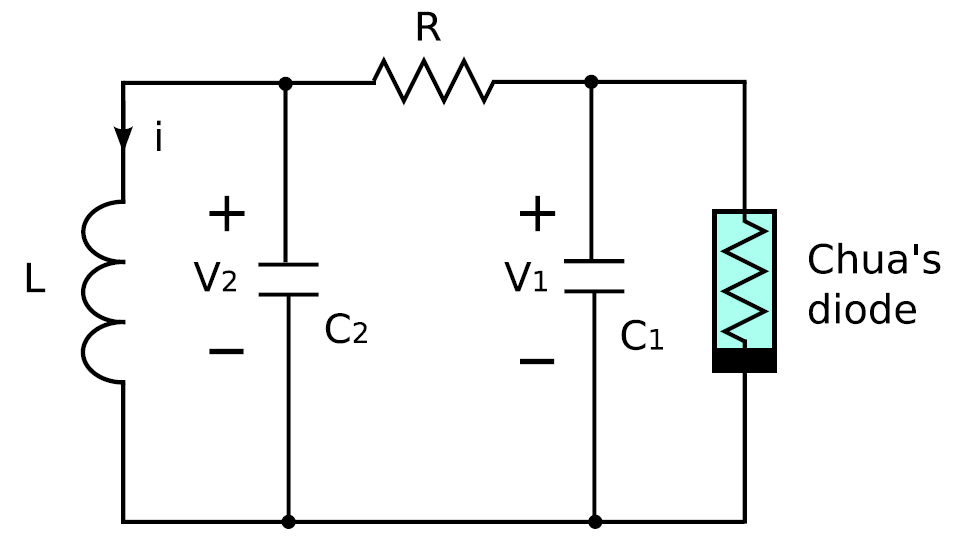
\includegraphics[scale=0.25]{ChuaCircuit.png}
    \caption{Circuito de Chua \cite{Itoh2008}}
    \label{Fig:ChuaCircuit}
\end{figure}

Donde $f(x)$ corresponde a \ref{Eq:ChuaDiode} y bajo $\beta=1$ recuperamos el modelo usual presentada en \cite{Chua1994} . Mediante los parámetros $(\alpha\!=\!15.6 \,,\, \beta\!=\!1 \,,\, \gamma\!=\!28 \,,\, m_1\!=\!m_3\!=\!-0.714 \,,\, m_2\!=\!-1.143 \,,\, x_1\!=\!-1 \,,\, x_2\!=\!1 \,,\, \epsilon\!=\!0)$, sugeridos en \cite{ChuaCircuitSimulator}, y las condiciones iniciales ($x=0.7\,,\,y=0\,,\,z=0$) se obtiene el atractor de Chua presentado en la \textbf{Fig.} \ref{Fig:ChuaCircuit3D}

\begin{figure}[H]
    \centering
    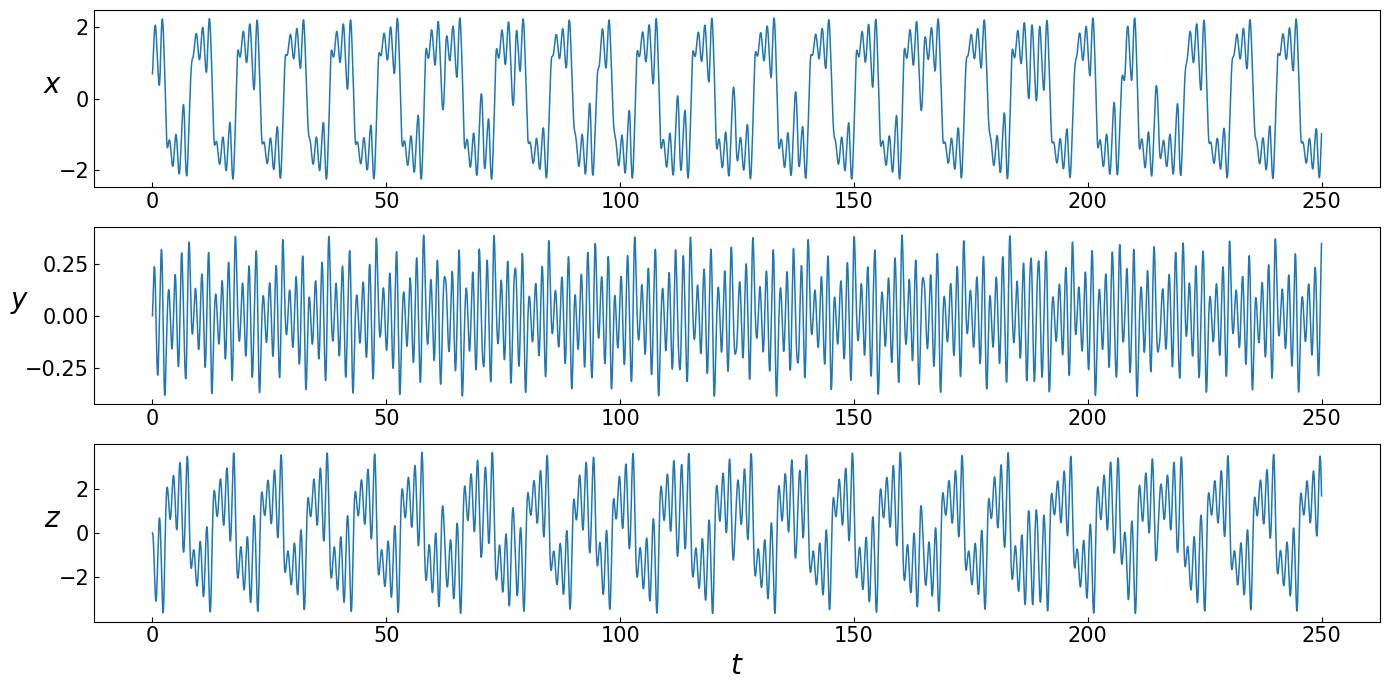
\includegraphics[scale=0.245]{ChuaOscillator1D.png}
    \caption{Evolución temporal del sistema \ref{Eq:ChuaCircuitA}}
    \label{Fig:ChuaCircuit1D}
\end{figure}

\begin{figure}[H]
    \centering
    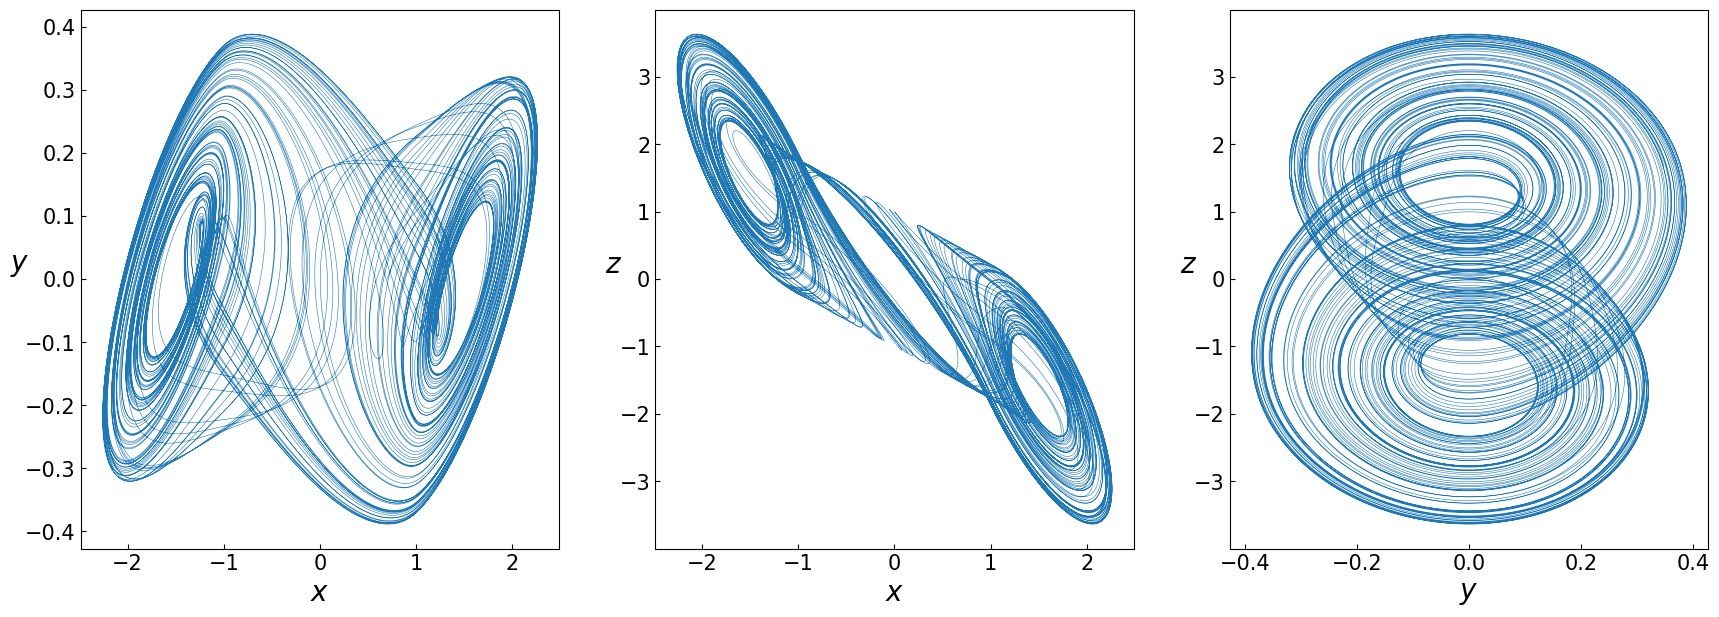
\includegraphics[scale=0.205]{ChuaOscillator2D.png}
    \caption{Proyección del atractor de Chua en los tres posibles planos}
    \label{Fig:ChuaCircuit2D}
\end{figure}

\begin{figure}[H]
    \centering
    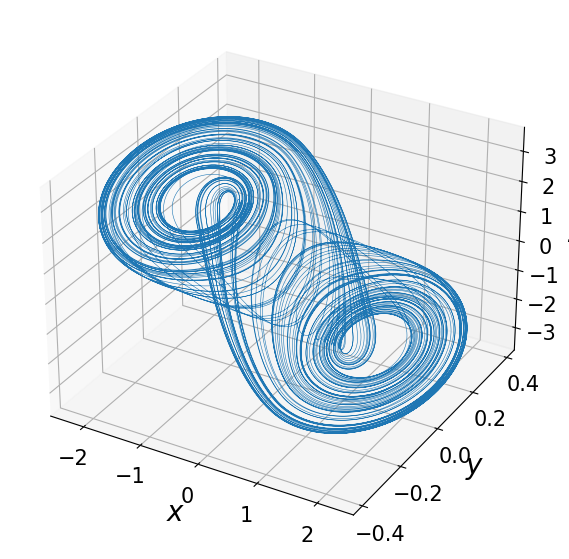
\includegraphics[scale=0.38]{ChuaOscillator3D.png}
    \caption{Atractor de Chua obtenido de \ref{Eq:ChuaCircuitA}}
    \label{Fig:ChuaCircuit3D}
\end{figure}

\subsection*{Oscilador de Van der Pol mediante un memristor}

Omitiremos el estudio del oscilador de Van der Pol y de su versión que emplea un diodo de Chua, presentada en la \textbf{Fig.} \ref{Fig:DiodeVanderPol}, en su lugar reemplazaremos en este ultimo el diodo de Chua por un memristor activo como se muestra en la \textbf{Fig} \ref{Fig:MemVanderPol}. Las ecuaciones de estado adimensionales que rigen este sistema son 

\begin{align}
\label{Eq:MemVanderPol}
&\frac{dx}{dt} = \alpha\bigg[- y - x\cdot W\big(z\big) + \gamma x\bigg] \nonumber \\ 
&\frac{dy}{dt} = \beta x \\
&\frac{dz}{dt} = x \nonumber 
\end{align}

\begin{figure}[H]
    \centering
    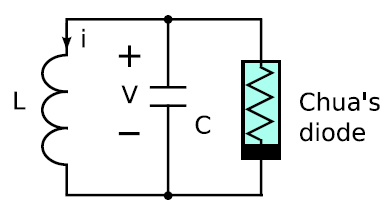
\includegraphics[scale=0.3]{DiodeVanderPol.png}
    \caption{Oscilador de Van der Pol empleando un diodo de Chua \cite{Itoh2008}}
    \label{Fig:DiodeVanderPol}
\end{figure}

\begin{figure}[H]
    \centering
    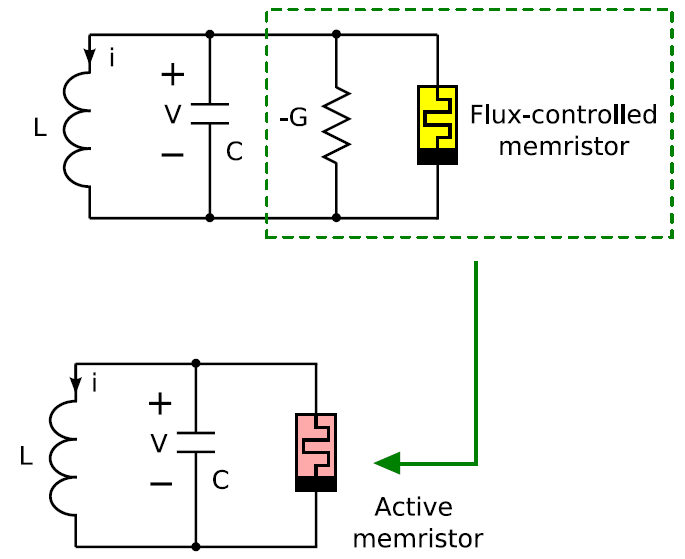
\includegraphics[scale=0.25]{MemVanderPol.png}
    \caption{Oscilador de Van der Pol empleando un memristor activo \cite{Itoh2008}}
    \label{Fig:MemVanderPol}
\end{figure}

Donde $W$ es la memductancia de un memristor monótonamente-creciente y lineal a trozos discutido previamente. Las ecuaciones dimensionales del sistema se encuentran en \cite{Itoh2008}, allí también se sugieren los parámetros $(\alpha\!=\!2 \,,\, \beta\!=\!1 \,,\, \gamma\!=\!0.3 \,,\, a\!=\!0.1 \,,\, b\!=\!0.5)$, con ellos y junto a las condiciones iniciales ($x\!=\!0.25\,,\,y\!=\!0\,,\,z\!=\!0$) encontramos uno de los dos atractores que se mencionan en el paper (\textbf{Fig.} \ref{Fig:MemVanderPol3D})

\begin{figure}[H]
    \centering
    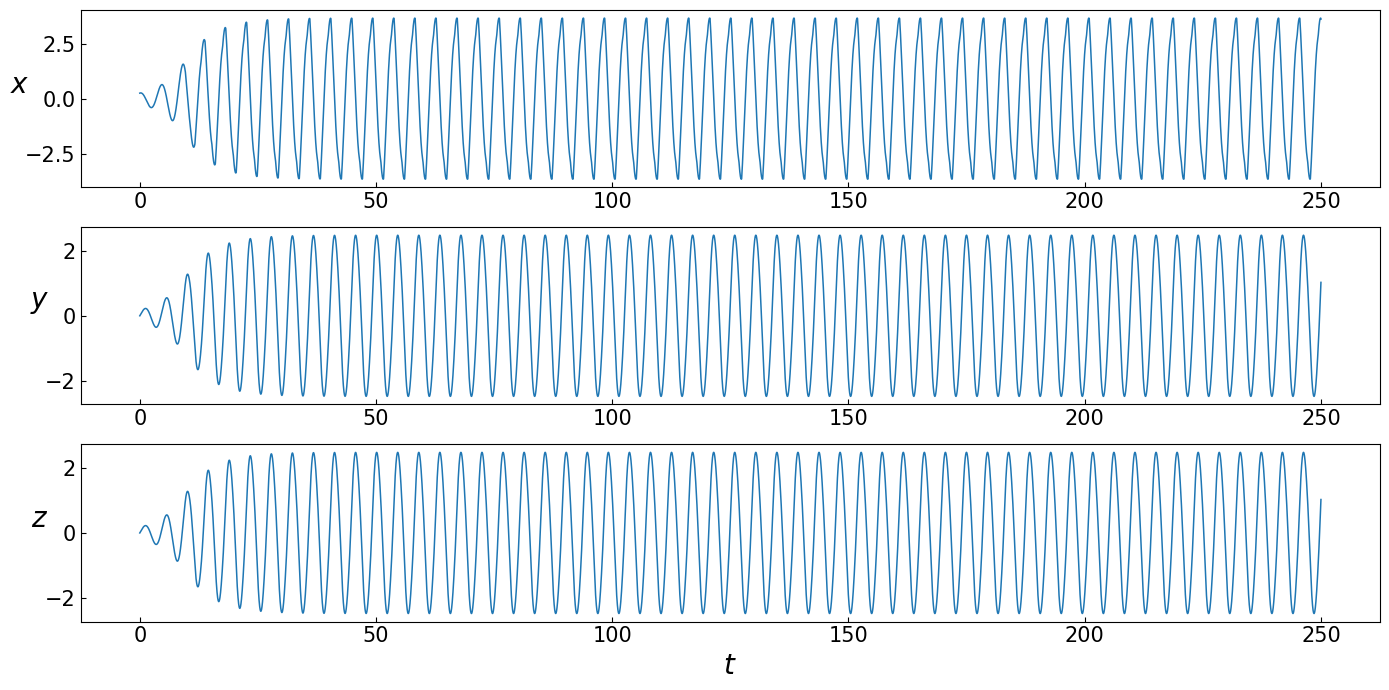
\includegraphics[scale=0.245]{Memristor-basedVanderPolOscillator1D.png}
    \caption{Evolución temporal del sistema \ref{Eq:MemVanderPol}}
    \label{Fig:MemVanderPol1D}
\end{figure}

\begin{figure}[H]
    \centering
    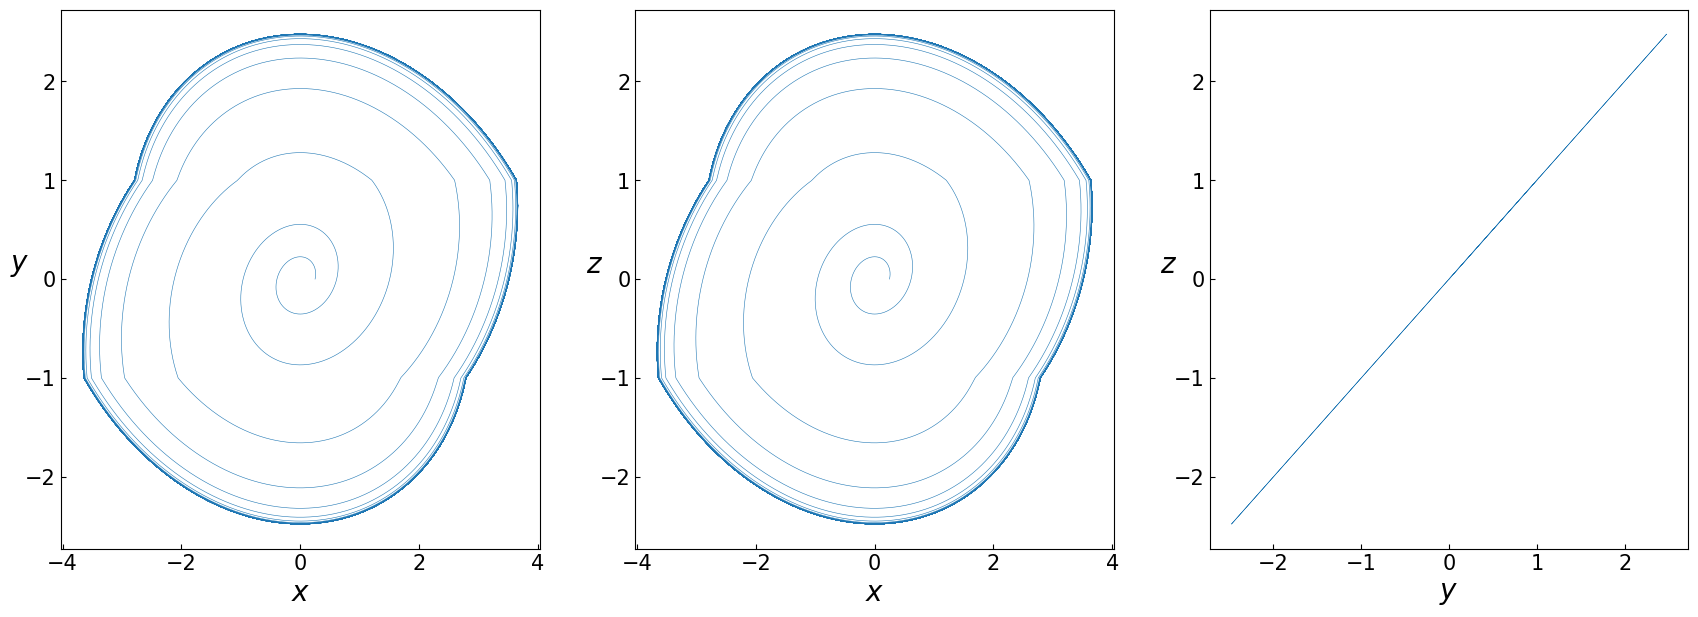
\includegraphics[scale=0.205]{Memristor-basedVanderPolOscillator2D.png}
    \caption{Proyecciones sobre los planos de la trayectoria de fase}
    \label{Fig:MemVanderPol2D}
\end{figure}

\begin{figure}[H]
    \centering
    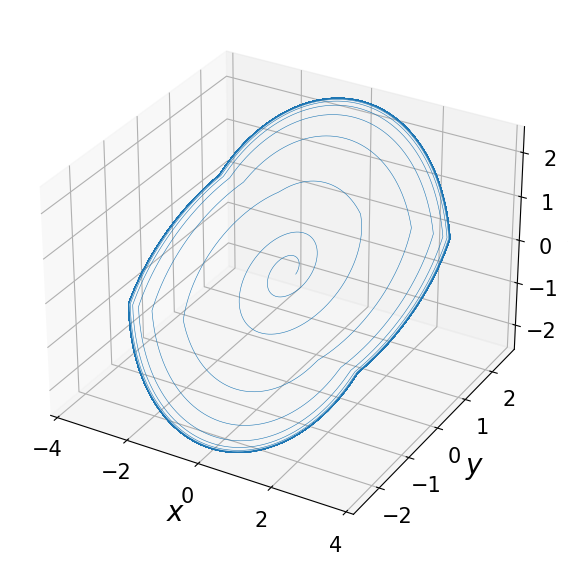
\includegraphics[scale=0.38]{Memristor-basedVanderPolOscillator3D.png}
    \caption{Atractor encontrado para \ref{Eq:MemVanderPol}}
    \label{Fig:MemVanderPol3D}
\end{figure}


\subsection*{Oscilador de Chua mediante un memristor}
Ahora lidiaremos con un oscilador de Chua (Ver la \textbf{Fig.} \ref{Fig:ChuaOscilator} para su versión original) que incorpora un memristor en el lugar del diodo de Chua, ilustrada en la \textbf{Fig.} \ref{Fig:MemChuaOscilator}. Aplicando las leyes de Kirchhoff y mediante un proceso de adimensionalizacion obtenemos el sistema propuesto en \cite{Itoh2008}

\begin{align}
\begin{split}
\label{Eq:MemChuaOscilator}
&\frac{dx}{dt} = \alpha\bigg[y - x +\xi x - x\cdot W\big(u\big)\bigg] \\ 
&\frac{dy}{dt} = x - y + z  \\
&\frac{dz}{dt} = -\beta y -\gamma z  \\
&\frac{du}{dt} = x 
\end{split}
\end{align}

\begin{figure}[H]
    \centering
    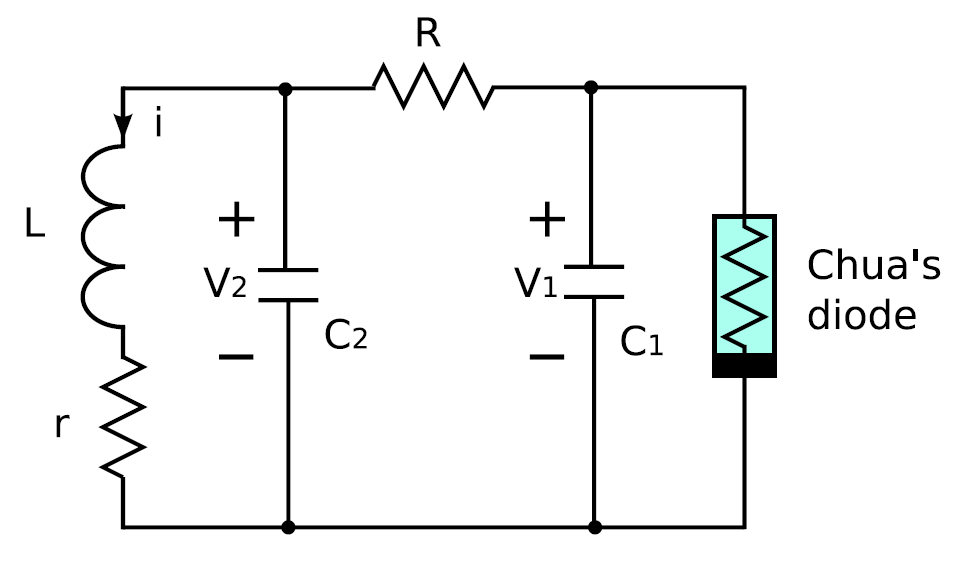
\includegraphics[scale=0.25]{ChuaOscilator.png}
    \caption{Oscilador de Chua \cite{Itoh2008}}
    \label{Fig:ChuaOscilator}
\end{figure}

\begin{figure}[H]
    \centering
    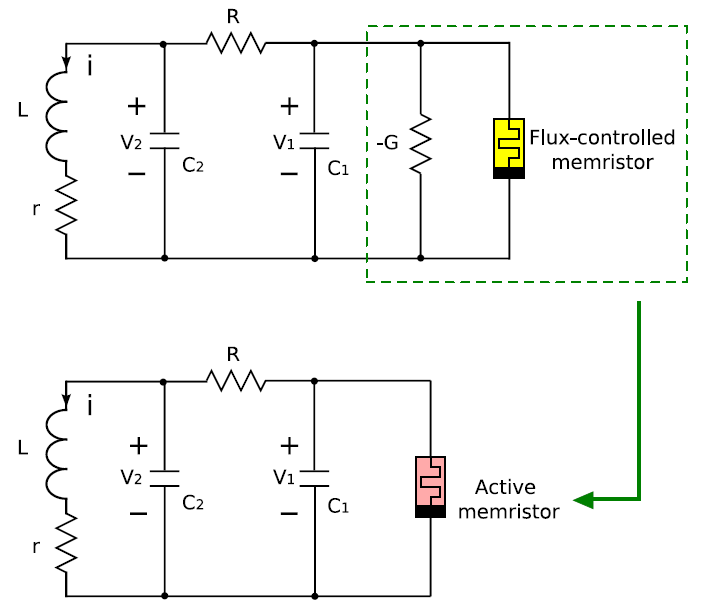
\includegraphics[scale=0.25]{MemChuaOscilator.png}
    \caption{Oscilador de Chua empleando un memristor activo \cite{Itoh2008}}
    \label{Fig:MemChuaOscilator}
\end{figure}


Utilizando los parámetros sugeridos $(\alpha\!=\!10 \,,\, \beta\!=\!13 \,,\, \gamma\!=\!0.35 \,,\, \xi\!=\!1.5 \,,\,a\!=\!0.3 \,,\, b\!=\!0.8)$ y con las condiciones iniciales ($x\!=\!0.25\,,\,y\!=\!0\,,\,z\!=\!0$) logramos replicar la evolución temporal y las proyecciones en dos dimensiones presentadas en \cite{Buscarino2012a} y las proyecciones en tres dimensiones expuestas en \cite{Itoh2008} 

\begin{figure}[H]
    \centering
    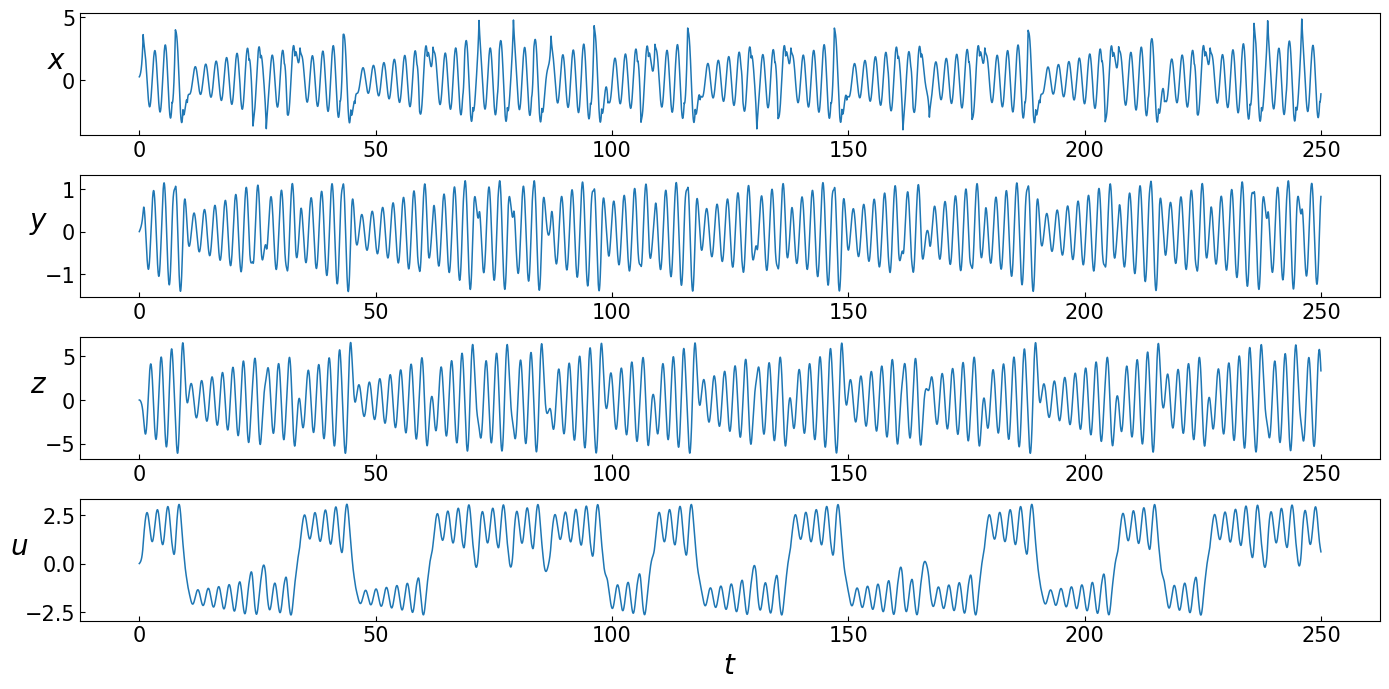
\includegraphics[scale=0.245]{Memristor-basedChuaOscillator1D.png}
    \caption{Evolución temporal del sistema \ref{Eq:MemChuaOscilator}}
    \label{Fig:ChuaCircuit1D}
\end{figure}

\begin{figure}[H]
    \centering
    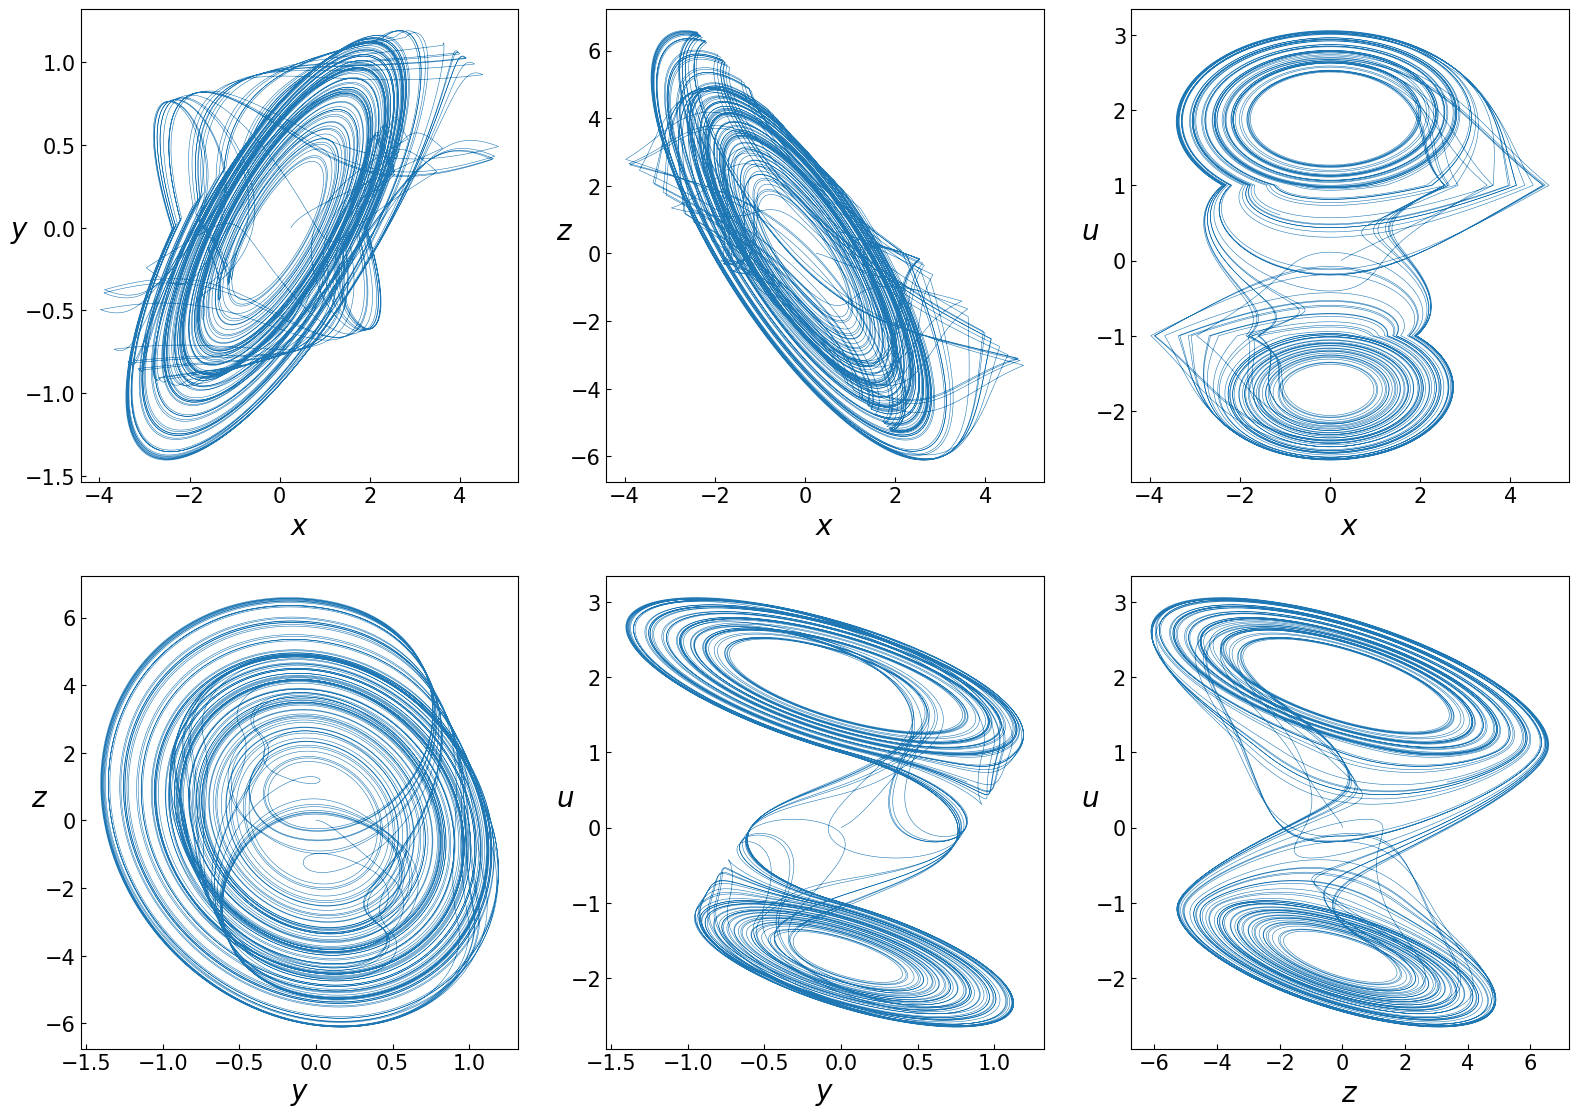
\includegraphics[scale=0.205]{Memristor-basedChuaOscillator2Dv2.png}
    \caption{Proyecciones en dos dimensiones de las trayectoria fasica}
    \label{Fig:ChuaCircuit2D}
\end{figure}

\begin{figure}[H]
    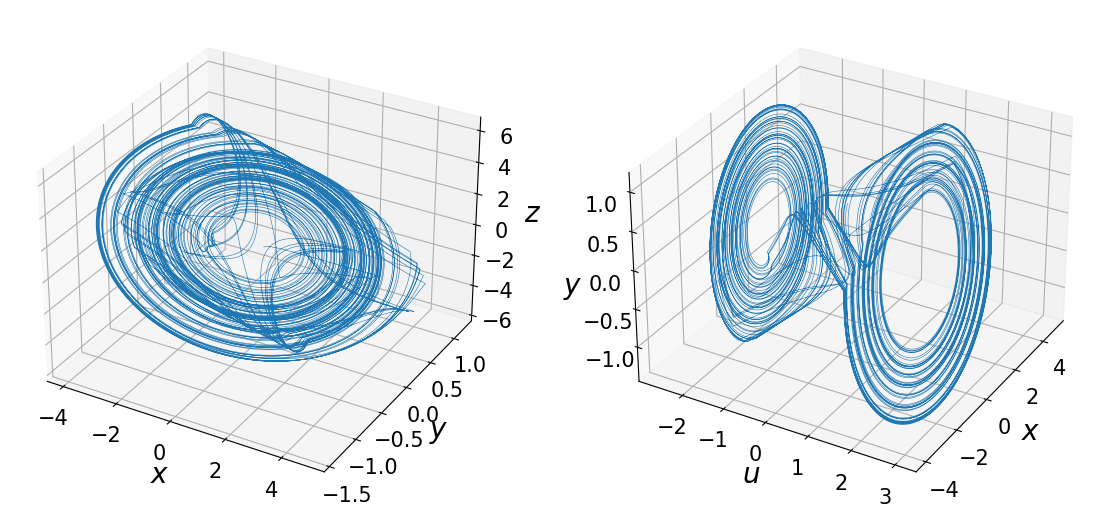
\includegraphics[scale=0.32]{Memristor-basedChuaOscillator3D.png}
    \caption{Proyecciones en tres dimensiones de la trayectoria fasica, donde se observa un atractor}
    \label{Fig:ChuaCircuit3D}
\end{figure}

\subsection*{Oscilador Canónico de Chua mediante un Memristor}

Al cambiar el diodo de Chua en un oscilador canónico de Chua (Ver \textbf{Fig.} \ref{Fig:CanonChuaOscilator}) se obtiene un sistema (Ver \textbf{Fig.} \ref{Fig:MemCanonChuaOscilator}) regido por el sistema de ecuaciones 

\begin{align}
\begin{split}
\label{Eq:MemCanChuaOscilator}
&\frac{dx}{dt} = \alpha\bigg[y - x\cdot W\big(u\big)\bigg] \\ 
&\frac{dy}{dt} = z - x   \\
&\frac{dz}{dt} = -\beta y + \gamma z \\
&\frac{du}{dt} = x
\end{split}
\end{align}

\begin{figure}[H]
    \centering
    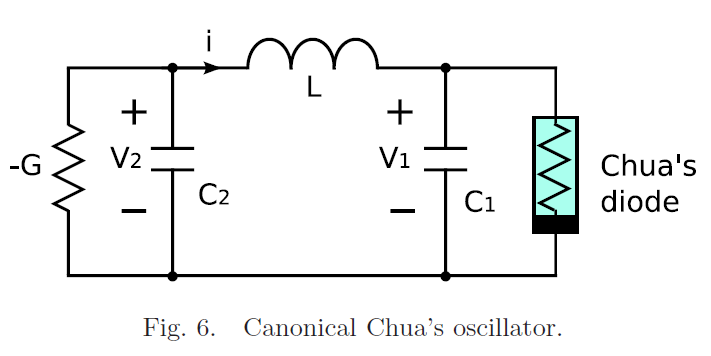
\includegraphics[scale=0.25]{CanChuaOscilator.png}
    \caption{Oscilador canónico de Chua \cite{Itoh2008}}
    \label{Fig:CanonChuaOscilator}
\end{figure}

\begin{figure}[H]
    \centering
    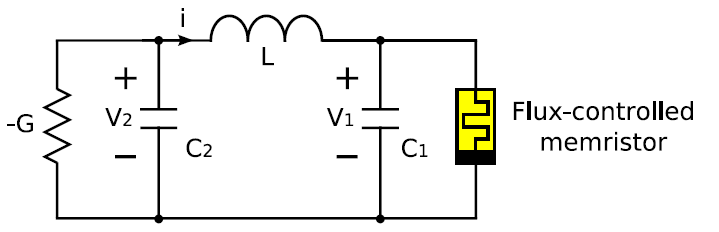
\includegraphics[scale=0.25]{MemCanChuaOscilator.png}
    \caption{Oscilador canónico de Chua empleando un memristor controlado por flujo \cite{Itoh2008}}
    \label{Fig:MemCanonChuaOscilator}
\end{figure}

Utilizando los parámetros sugeridos $(\alpha\!=\!4 \,,\, \beta\!=\!1 \,,\, \gamma\!=\!0.65 \,,\,a\!=\!0.2 \,,\, b\!=\!10)$ y con las condiciones iniciales ($x\!=\!0.25\,,\,y\!=\!0\,,\,z\!=\!0$) logramos replicar la evolución temporal y las proyecciones en dos dimensiones presentadas en \cite{Buscarino2012a} y las proyecciones en tres dimensiones expuestas en \cite{Itoh2008} 

\begin{figure}[H]
    \centering
    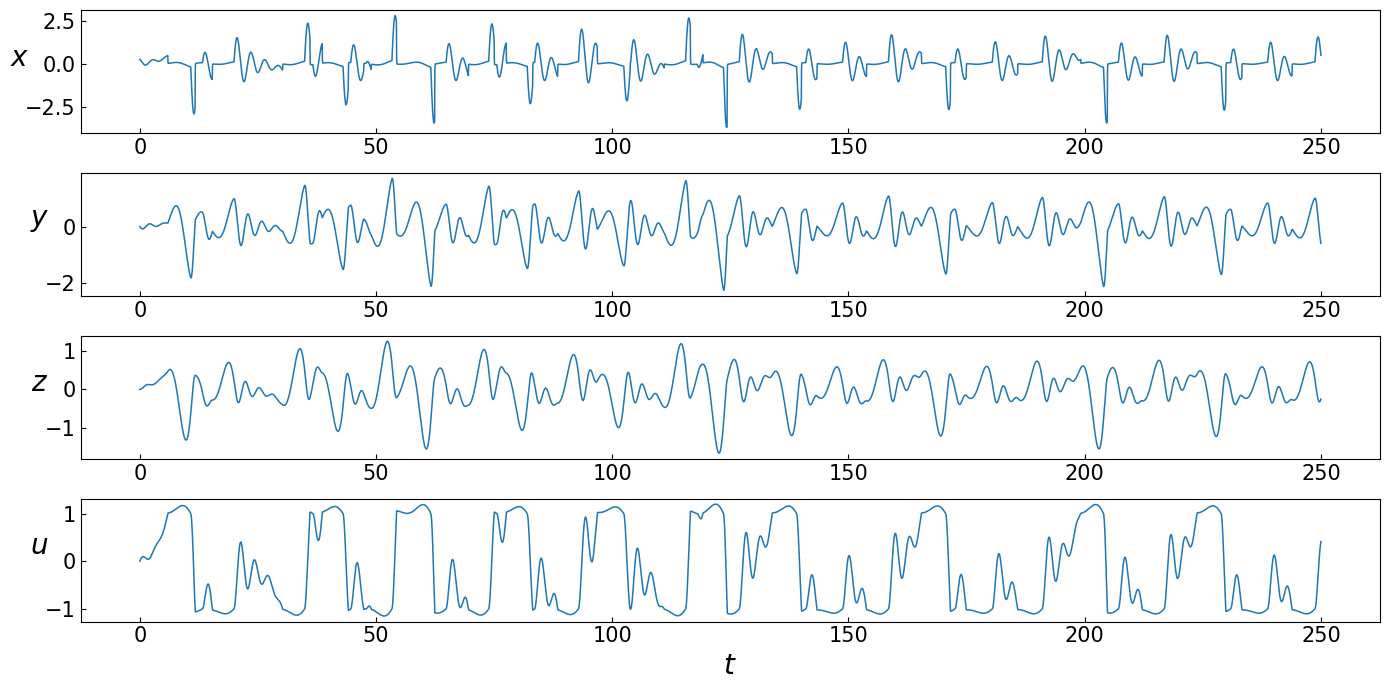
\includegraphics[scale=0.245]{Memristor-basedCanonicalChuaOscillator1D.png}
    \caption{Evolución temporal del sistema \ref{Eq:MemCanChuaOscilator}}
    \label{Fig:MemCanChuaOscilator1D}
\end{figure}

\begin{figure}[H]
    \centering
    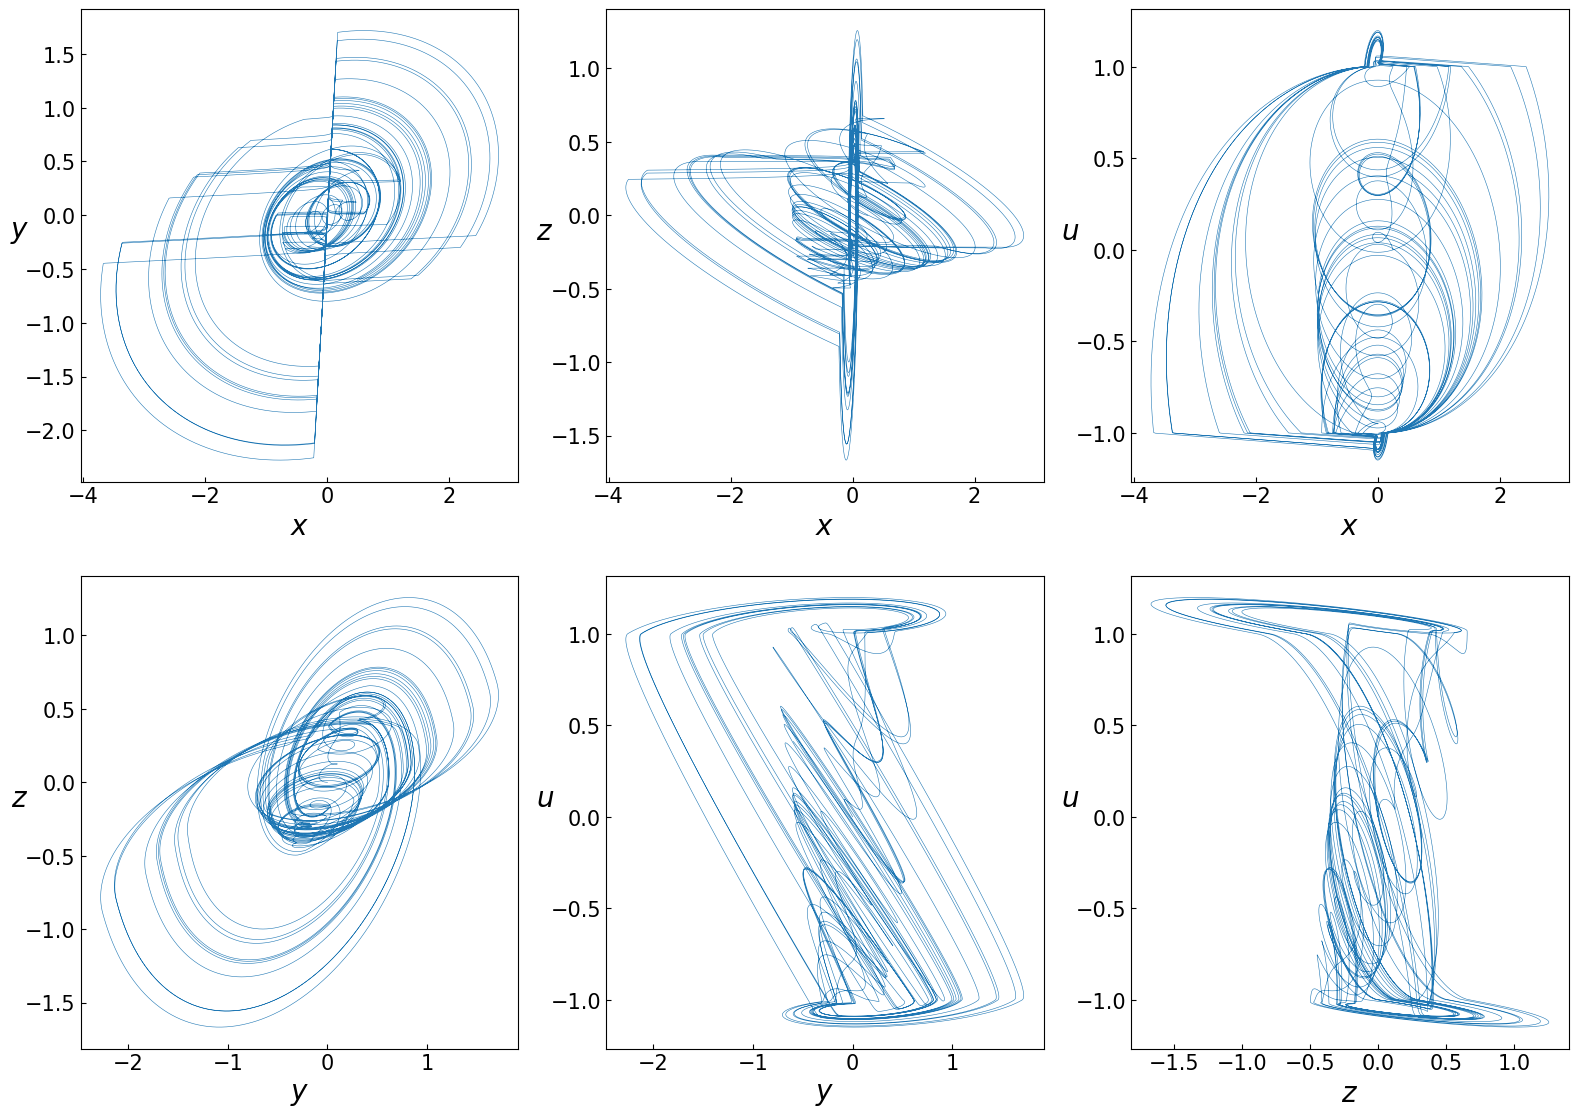
\includegraphics[scale=0.205]{Memristor-basedCanonicalChuaOscillator2Dv2.png}
    \caption{Proyecciones en dos dimensiones de las trayectoria fasica}
    \label{Fig:MemCanChuaOscilator2D}
\end{figure}

\begin{figure}[H]
    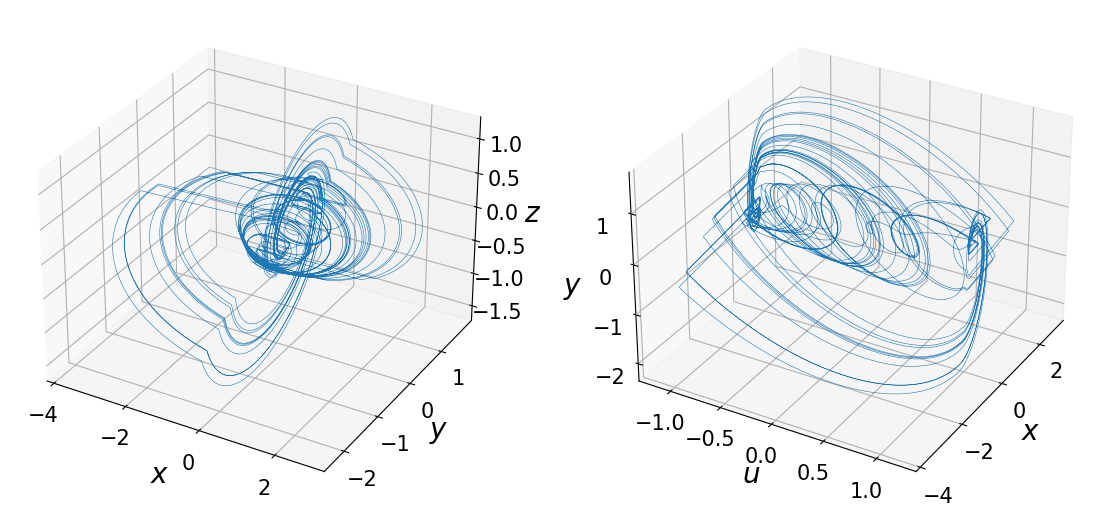
\includegraphics[scale=0.32]{Memristor-basedCanonicalChuaOscillator3D.png}
    \caption{Proyecciones en tres dimensiones de la trayectoria fasica, donde se observa un atractor}
    \label{Fig:MemCanChuaOscilator3D}
\end{figure}

Removiendo la resistencia en paralelo con el capacitor obtenemos el circuito de la \textbf{Fig.} \ref{Fig:ModCanChuaOscilator}. La dinámica del sistema esta descrita por \ref{Eq:ModCanChuaOscilator}

\begin{align}
\begin{split}
\label{Eq:ModCanChuaOscilator}
&\frac{dx}{dt} = \alpha\bigg[y - x\cdot W\big(u\big)\bigg] \\ 
&\frac{dy}{dt} = -\xi(x+z)  \\
&\frac{dz}{dt} = \beta y  \\
&\frac{du}{dt} = x
\end{split}
\end{align}


\begin{figure}[H]
    \centering
    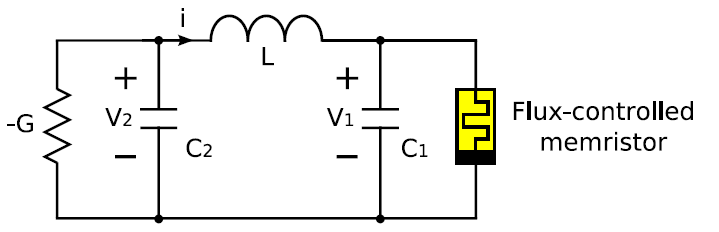
\includegraphics[scale=0.25]{MemCanChuaOscilator.png}
    \caption{Oscilador canónico de Chua empleando un memristor controlado por flujo \cite{Itoh2008}}
    \label{Fig:ModCanChuaOscilator}
\end{figure}

Utilizando los parámetros sugeridos $(\alpha\!=\!4.2 \,,\, \beta\!=\!-20 \,,\, \xi\!=\!-1 \,,\,a\!=\!-2 \,,\, b\!=\!9)$ y con las condiciones iniciales ($x\!=\!0.25\,,\,y\!=\!0\,,\,z\!=\!0$) obtenemos la evolución temporal y las proyecciones en dos dimensiones del sistema y replicamos las proyecciones en tres dimensiones expuestas en \cite{Itoh2008} 

\begin{figure}[H]
    \centering
    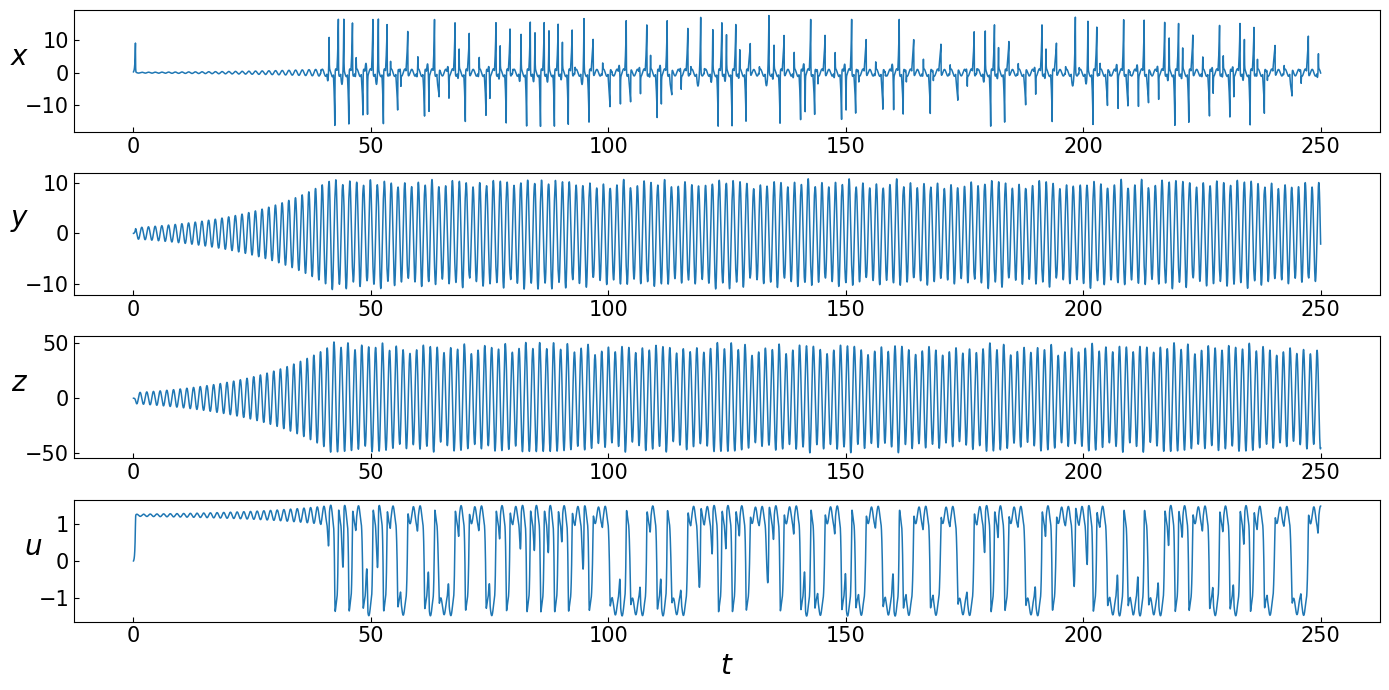
\includegraphics[scale=0.245]{ModifiedMemristor-basedCanonicalChuaOscillator1D.png}
    \caption{Evolución temporal del sistema \ref{Eq:MemChuaOscilator}}
    \label{Fig:MemCanChuaOscilator1D}
\end{figure}

\begin{figure}[H]
    \centering
    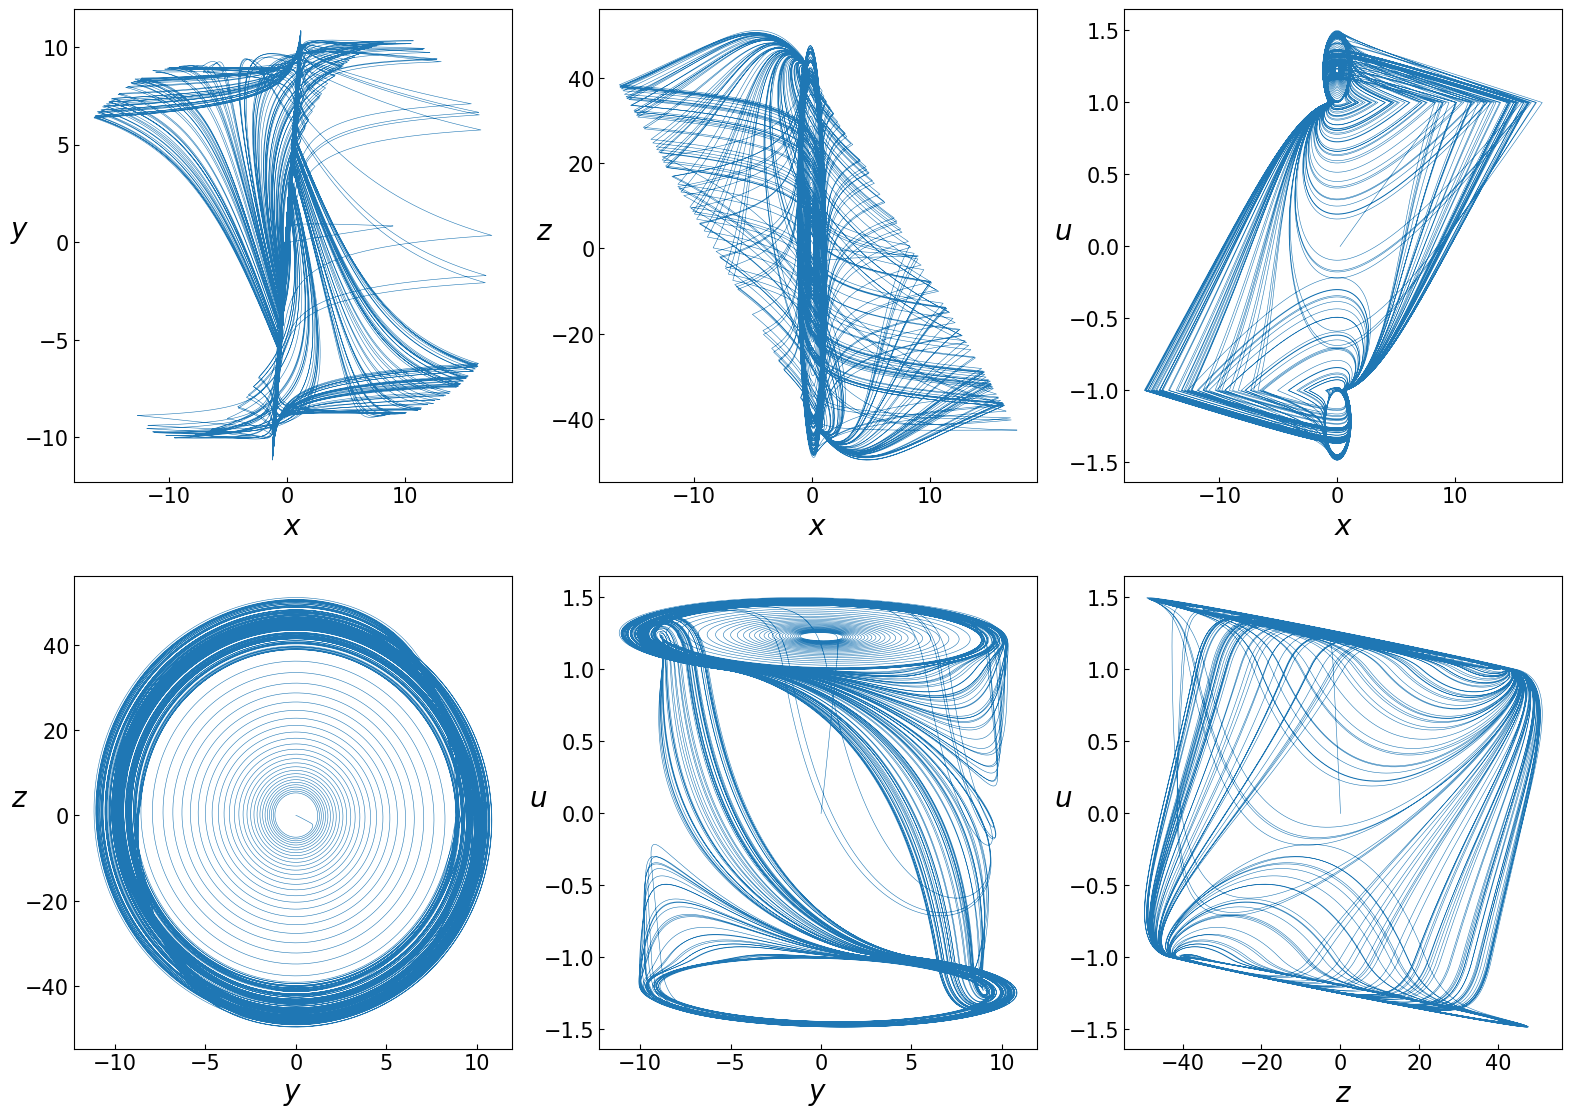
\includegraphics[scale=0.205]{ModifiedMemristor-basedCanonicalChuaOscillator2Dv2.png}
    \caption{Proyecciones en dos dimensiones de las trayectoria fasica}
    \label{Fig:MemCanChuaOscilator2D}
\end{figure}

\begin{figure}[H]
    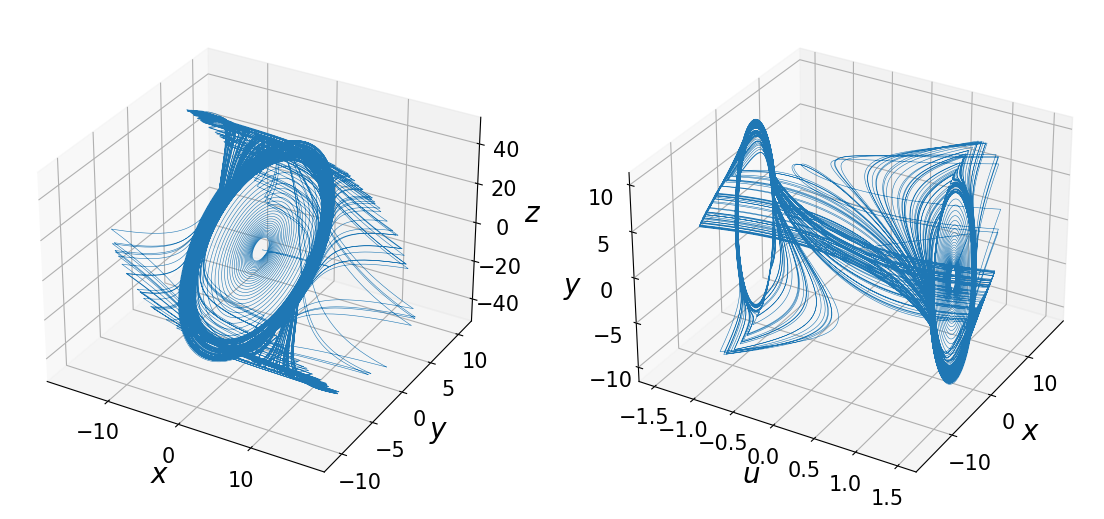
\includegraphics[scale=0.32]{ModifiedMemristor-basedCanonicalChuaOscillator3D.png}
    \caption{Proyecciones en tres dimensiones de la trayectoria fasica, donde se observa un atractor}
    \label{Fig:MemCanChuaOscilator3D}
\end{figure}

\section*{Complejidad Emergente en Redes Celulares Neuronales}

Una vez explorados los circuitos caóticos quisimos replicar los resultados de \cite{Pham2012}\cite{Buscarino2016}\cite{Buscarino2018}, donde utilizan como célula el oscilador de Van der Pol de la \textbf{Fig.} \ref{Eq:MemVanderPol}.
A partir de la forma mas general de un sistema de acción difusión de dos capas 

\begin{align}
\begin{bmatrix}
   \dot{x} \\
   \dot{y}
\end{bmatrix}
=
\begin{bmatrix}
   D_{11} & D_{12} \\
   D_{21} & D_{22}
\end{bmatrix}
\begin{bmatrix}
   \nabla^2 x \\
   \nabla^2 y
\end{bmatrix}
+
\begin{bmatrix}
   f(x,y) \\
   g(x,y)
\end{bmatrix}
\end{align}

Se plantea un sistema donde los componente de reacción están dados por las funciones que definen el sistema \ref{Eq:MemVanderPol}, pero se escribe explícitamente una ecuación para $z$ para no perder de vista el comportamiento de este basado en las condiciones iniciales.

\begin{align}
\label{Eq:ReactionDiffusion}
&\dot{x} = D_{11} \nabla^2 x + D_{12} \nabla^2 y + \alpha\bigg[ - y - x W\big( z\big) + \gamma x \bigg] \nonumber \\
&\dot{y} = D_{21} \nabla^2 x + D_{22} \nabla^2 y + \beta x \\
&\dot{z} = x \nonumber
\end{align}

El primer fenómeno a explorar es el de las llamadas "\textit{autowaves}", para que nuestro sistema genere este comportamiento es necesario a su vez que sea capaz de exhibir "\textit{slow-fast dynamics}" \cite{Perez1993}\cite{Arena1997}característica de varios sistemas biológicos. Afortunadamente este puede obtener mediante los parámetros $(\alpha\!=\!10 \,,\, \beta\!=\!0.01 \,,\, \gamma\!=\!0.3\,,\,a\!=\!0.1 \,,\, b\!=\!0.5)$, en la \textbf{Fig.} \ref{Fig:SlowFastDynamics} puede observarse la evolución temporal del sistema bajo las condiciones iniciales ($x=0.25\,,\,y=0\,,\,z=0$).

\begin{figure}[H]
    \centering
    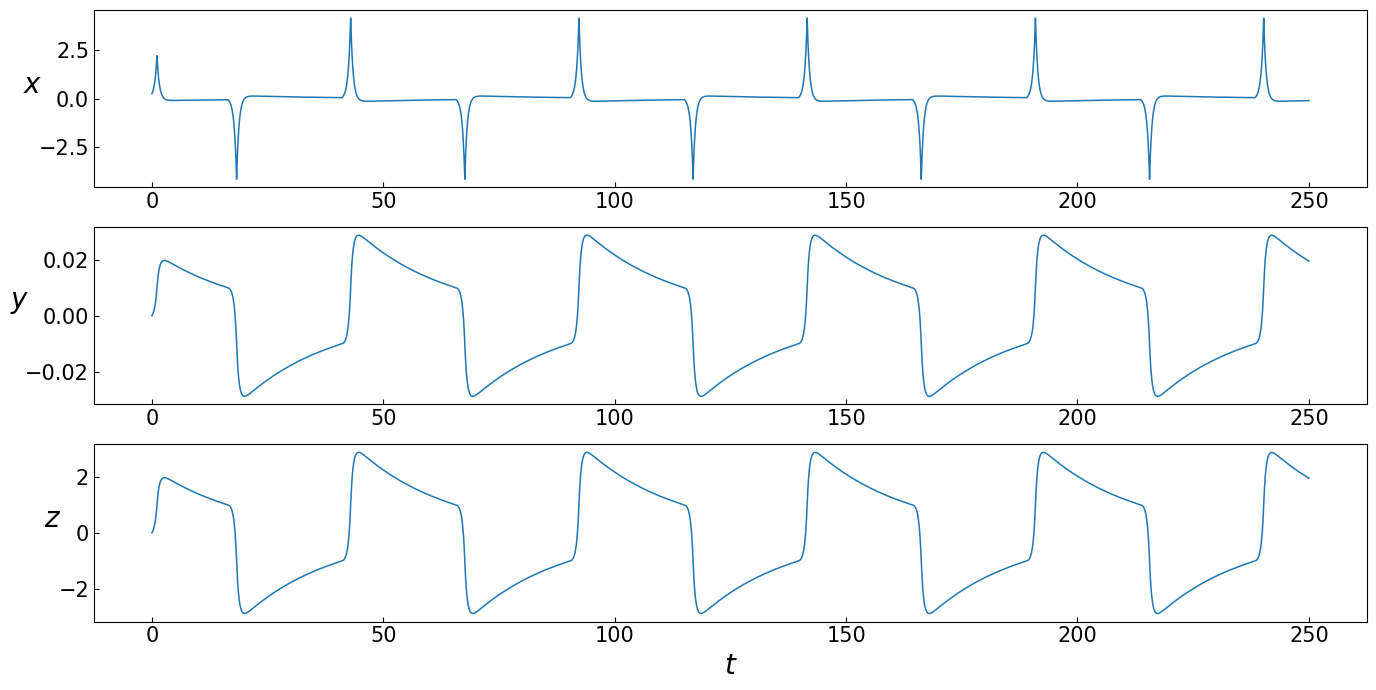
\includegraphics[scale=0.245]{SlowFastDynamicsMemVanderPolOscilator.png}
    \caption{El oscilador de Van der Pol puede exhibir dinámica "\textit{slow-fast}" \ref{Eq:MemChuaOscilator}}
    \label{Fig:MemCanChuaOscilator1D}
\end{figure}

Siguiendo \cite{Pham2012} simulamos el caso $(D_{12}\!=\!D_{21}\!=\!D_{22}\!=\!0 \,,\,  \alpha\!=\!10 \,,\,\beta\!=\!0.01 \,,\, \gamma\!=\!0.3\,,\,a\!=\!0.1 \,,\, b\!=\!0.5)$ con condiciones Neumann homogéneas en las fronteras, mediante las formulas recursivas \ref{Eq:Autowaves} e imponiendo la condición $x_{ij}=1.5$ de manera apropiada para replicar los resultados deseados. Observe que el laplaciano empleado es totalmente local y no emplea términos como $dx$ o $dy$, la naturaleza de esta elección no es del toda clara para nosotros por el momento.

\begin{align}
\label{Eq:Autowaves}
x^{n+1}_{i,j} &= x^{n}_{i,j} + dt\,D_{11}\nabla^2 x \nonumber \\
                +& \alpha\,dt\bigg[ - y^{n}_{i,j} - x^{n}_{i,j}\cdot W\big(Z^{n}_{i,j}\big) + \gamma x^{\,n}_{i,j} \bigg] \nonumber\\
y^{n+1}_{i,j} &= y^{n}_{i,j}  + \beta\,dt\,x^{n}_{i,j} \\
z^{n+1}_{i,j} &= z^{n}_{i,j} + dt\,x^{\,n}_{i,j} \nonumber
\end{align} 

\begin{figure}[H]
    \centering
    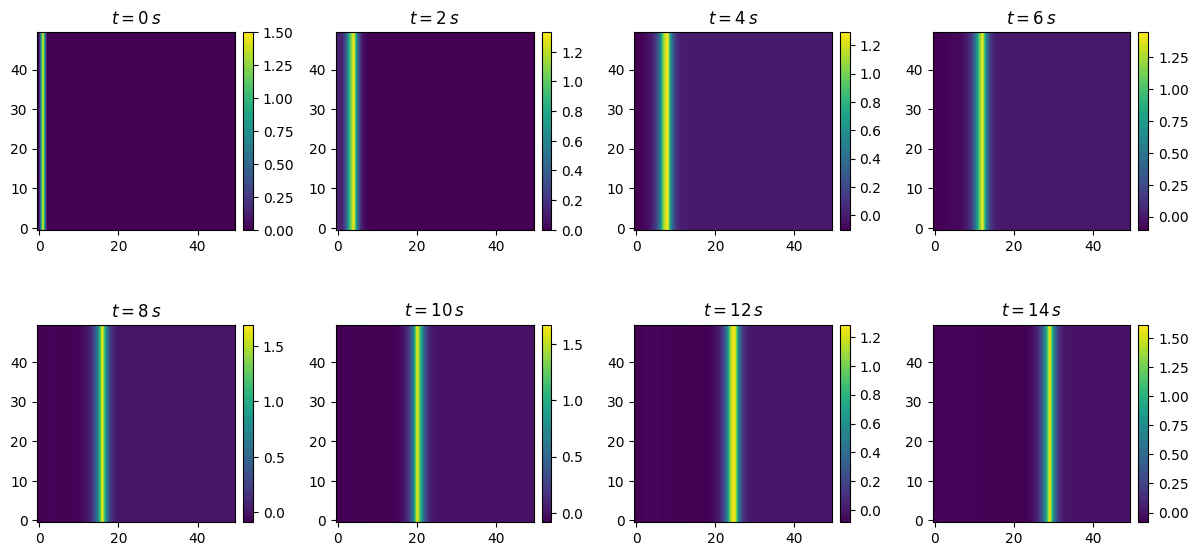
\includegraphics[scale=0.27]{PlaneWave.png}
    \caption{Onda plana viajera}
    \label{Fig:PlaneWave}
\end{figure}

\begin{figure}[H]
    \centering
    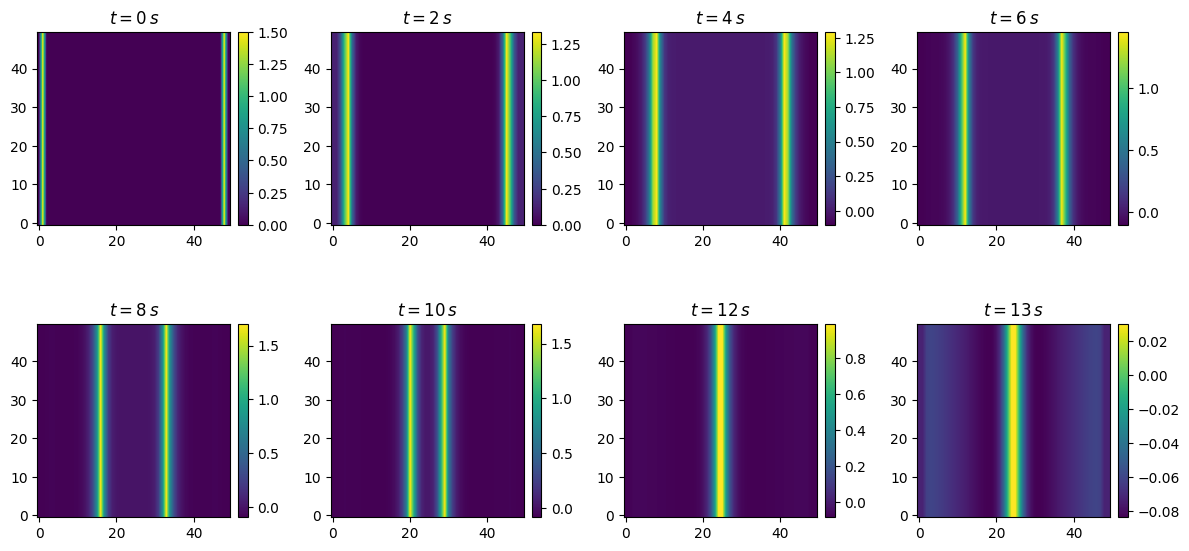
\includegraphics[scale=0.27]{PlaneWaves.png}
    \caption{Ondas planas viajeras paralelas. No se replica la aniquilación deseada, pero no difiere mucho de esta}
    \label{Fig:PlaneWaves}
\end{figure}

\begin{figure}[H]
    \centering
    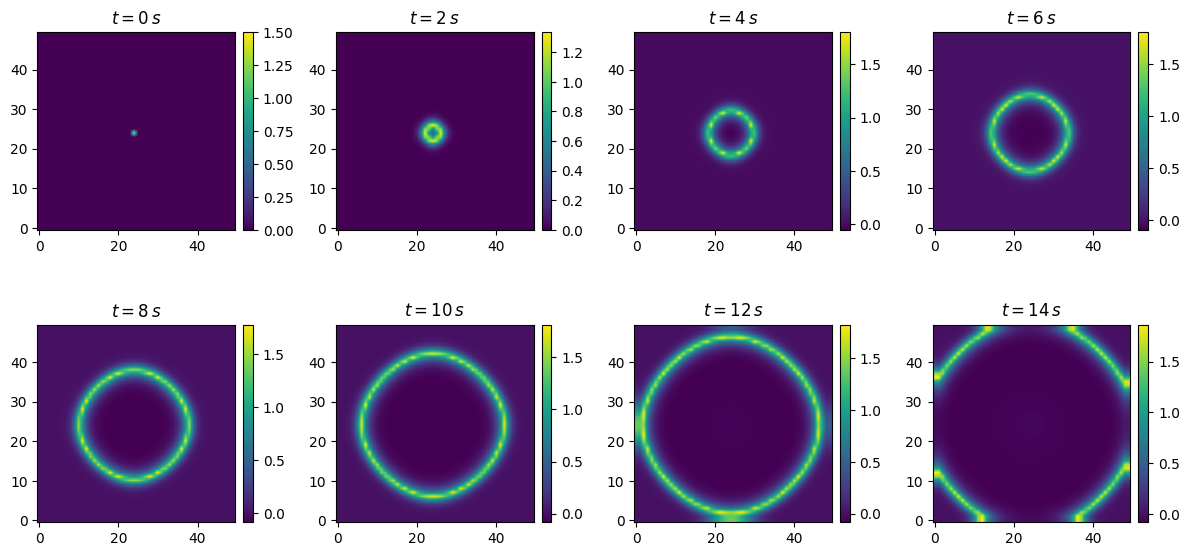
\includegraphics[scale=0.27]{SphericalWave.png}
    \caption{Onda esférica viajera}
    \label{Fig:SphericalWave}
\end{figure}

\begin{figure}[H]
    \centering
    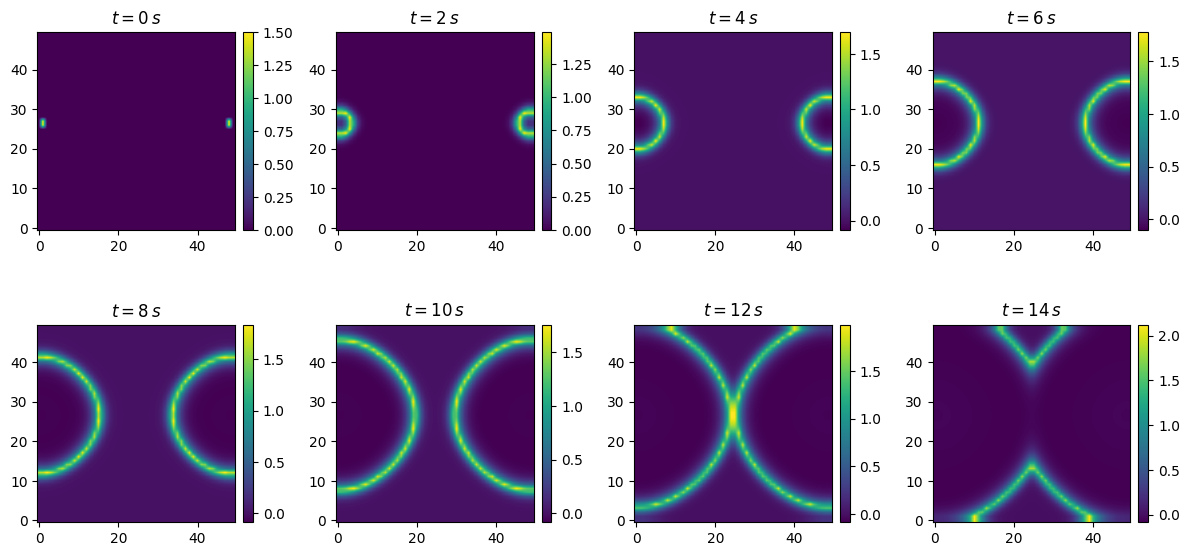
\includegraphics[scale=0.27]{SphericalWaves.png}
    \caption{Aniquilación de dos ondas esféricas viajeras}
    \label{Fig:SphericalWaves}
\end{figure}

Finalmente si no despreciamos ninguno de los coeficientes de difusión $D$ podemos satisfacer las condiciones para la inestabilidad de Turing. Seguiremos los casos estudiados en \cite{Buscarino2018}, donde se utiliza la dependencia lineal entre $\dot{y}$ y $\dot{z}$ para obtener un sistema de dos ecuaciones

\begin{align}
x^{n+1}_{i,j} &= X^{n}_{i,j} + dt\bigg[ D_{1,1} \nabla^2 x + D_{1,2} \nabla^2 y\bigg]  \nonumber\\
+  \alpha\,&dt\bigg[-y^{n}_{i,j} - x^{n}_{i,j}\cdot W\bigg(\frac{Y^{n}_{i,j}+C}{\beta}\bigg) + \gamma X^{n}_{i,j} \bigg] \\
y^{n+1}_{i,j} &= Y^{n}_{i,j} + dt\bigg[ D_{2,1} \nabla^2 x + D_{2,2} \nabla^2 y\bigg] + \beta\,dt\,x^{n}_{i,j} \nonumber
\end{align} 

El paper utiliza los valores $(D_{11}\!=\!1\,,\,D_{12}\!=\!4\,,\,D_{21}\!=\!6\,,\,D_{22}\!=\!26 \,,\,  \alpha\!=\!1 \,,\,\beta\!=\!0.8 \,,\, a\!=\!-0.01 \,,\, b\!=\!-0.61)$ Lamentablemente en el paper no se especifica el valor de $\gamma$ y por alguna razón hay un cambio de signo en el termino $xW(y/\beta + C)$. En parte debido a esto no fuimos capaces de reproducir los resultados, nuestras simulaciones se encuentran a continuación

\begin{figure}[H]
    \centering
    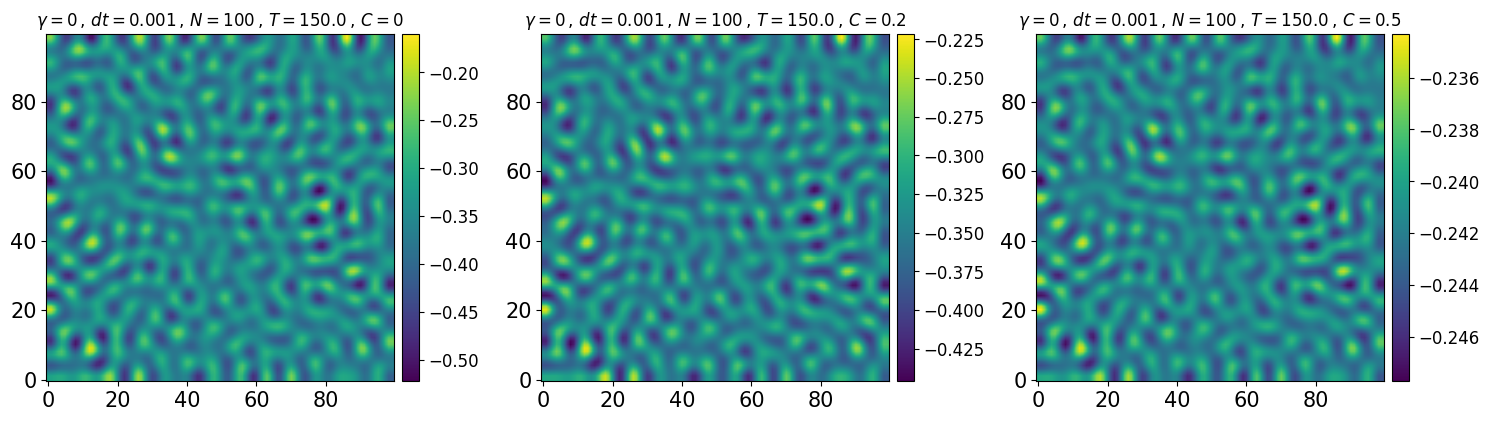
\includegraphics[scale=0.24]{Turing.png}
    \caption{Se observan características usuales de los patrones de Turing, pero no se replican los resultados del paper o siquiera la alta dependencia del parametro $C$}
    \label{Fig:SphericalWaves}
\end{figure}

\begin{thebibliography}{9}
\bibitem{Hodgkin1952} Hodkin A.L., Huxley, A.F. (1952). 'A quantitative description of membrane current and its application to conduction and excitation in nerve'. \textit{The Journal of physiology}. \textbf{117}(4), pp. 500–544.

\bibitem{FitzHugh1961} FitzHugh R. (1961). 'Impulses and Physiological States in Theoretical Models of Nerve Membrane'. \textit{Biophysical Journal}. \textbf{1}(6), pp. 445–466.

\bibitem{Nagumo1962} Nagumo J., Arimoto S., Yoshizawa S. (1962). 'An Active Pulse Transmission Line Simulating Nerve Axon'. \textit{Proceedings of the IRE}. \textbf{50}(10), pp. 2061–2070.

\bibitem{VanderPol1920} Van der Pol B. (1920). 'A theory of the amplitude of free and forced triode
vibrations', \textit{Radio Review}. \textbf{1}, pp. 701-710 and 754-762 .

\bibitem{Chua2012} Chua L.O., Sbitnev V., Kim H. (2012). 'Hodgkin-Huxley axon is made of memristors'. \textit{International Journal of Bifurcation and Chaos}.  \textbf{22}(3), 1230011 

\bibitem{Chua1971} Chua L.O. (1971). 'Memristor - The missing circuit element'. \textit{IEEE Transactions on Circuit Theory}.  \textbf{18}(5), pp. 507–519

\bibitem{Pham2012} Pham V.T., Buscarino A., Fortuna L., Frasca M. (2012). 'Autowaves in memristive cellular neural networks'. \textit{International Journal of Bifurcation and Chaos}. \textbf{22}(8), 1230027 

\bibitem{Buscarino2016} Buscarino A., Corradino C., Fortuna L., Frasca M., Chua L.O. (2016). 'Turing patterns in memristive cellular nonlinear networks'. \textit{IEEE Transactions on Circuits and Systems I: Regular Papers}. \textbf{63}(8), pp. 1222–1230 

\bibitem{Buscarino2018} Buscarino A., Corradino C., Fortuna L., Frasca M., Pham VT. (2018). 'A Memristor-Based Cell for Complexity'. In: Corinto F., Torcini A. (eds) \textit{Nonlinear Dynamics in Computational Neuroscience}. PoliTO Springer Series. pp. 133–141

\bibitem{Itoh2008} Itoh M., Chua L.O. (2008). 'Memristor oscillators'. \textit{International Journal of Bifurcation and Chaos}. \textbf{18}(11), pp. 3183–3206 

\bibitem{Buscarino2012a} Buscarino A.,  Fortuna L., Frasca M., Gambuzza L. V., Sciuto G. (2012). 'Memristive chaotic circuits based on cellular nonlinear networks'. \textit{International Journal of Bifurcation and Chaos}. \textbf{22}(3), 1250070

\bibitem{Buscarino2012b} Buscarino A., Fortuna L., Frasca M., Gambuzza L.V. (2012). 'A chaotic circuit based on Hewlett-Packard memristor'. \textit{Chaos: An Interdisciplinary Journal of Nonlinear Science}. \textbf{22}(2), 023136

\bibitem{Matsumoto1984} Matsumoto T. (1984) 'A chaotic attractor from Chua's circuit'. \textit{IEEE Transactions on Circuits and Systems}. \textbf{31}(12), pp. 1055-1058

\bibitem{Chua1994} Chua L.O. (1994) 'Chua's Circuit: An overview ten years later". \textit{Journal of Circuits, Systems and Computers}. \textbf{4}(2), pp. 117-159 

\bibitem{ChuaCircuitSimulator} 'Chua's circuit simulator'. Disponible en: \url{http://www.chuacircuits.com/sim.php}.

\bibitem{Perez1993} Perez-Munuzuri V., Perez-Villar V., Chua L.O. (1993). "Autowaves for image processing on a twodimensional
CNN array of excitable nonlinear circuits: flat and wrinkled labyrinths".  \textit{IEEE Transactions on Circuits and Systems I: Fundamental Theory and Applications}. \textbf{40}(3), pp. 174–181 

\bibitem{Arena1997} Arena P., Caponetto R., Fortuna L., Manganaro G. (1997). "Cellular neural networks to explore
complexity". \textit{Soft Computing}. \textbf{1}(3), pp. 120–136 

\end{thebibliography}  
\end{multicols*}
\end{document}
